\documentclass[aspectratio=169]{beamer}


\usepackage[utf8]{inputenx} % For æ, ø, å
\usepackage{csquotes}       % Quotation marks
\usepackage{microtype}      % Improved typography
\usepackage{amssymb}        % Mathematical symbols
\usepackage{mathtools}      % Mathematical symbols
\usepackage[absolute, overlay]{textpos} % Arbitrary placement
\setlength{\TPHorizModule}{\paperwidth} % Textpos units
\setlength{\TPVertModule}{\paperheight} % Textpos units
\usepackage{tikz}
\usetikzlibrary{overlay-beamer-styles}  % Overlay effects for TikZ

\usepackage{hyperref}
\usepackage{svg}

\usepackage{color, soul, xcolor} % Colored text and highlighting, respectively
\usepackage{tikz-cd} % For commutative diagrams
\usepackage{tikz-3dplot}
\usetikzlibrary{angles}
\RequirePackage{pgfplots}
\usepackage{mathtools}
\usepackage{answers}
\usepackage{setspace}
\usepackage{graphicx}
\usepackage{enumerate}
\usepackage{multicol}
\usepackage{mathrsfs}
\usepackage{amsmath,amsthm,amssymb}
\usepackage{marvosym,wasysym} %fucking smileys
\usepackage{float}
\usepackage{morefloats}
\usepackage{pgf,tikz}
\pgfplotsset{compat=1.15}
\usepackage{mathrsfs}
\usetikzlibrary{arrows}
\usepackage{subcaption}
\usepackage[most]{tcolorbox}
\tcbuselibrary{theorems}
\usepackage{fancyvrb}
\usepackage{longtable,booktabs}
\usepackage{stackrel}

\newcommand{\vecx}{\boldsymbol{\vec{x}}}
\newcommand{\vecf}{\boldsymbol{\vec{f}}}
\newcommand{\xdot}{\boldsymbol{\dot{\vec{x}}}}



\usetheme{UiB}

\definecolor{lighter_csu_green}{RGB}{60,133,77}
\newcommand\boldgreen[1]{\textcolor{lighter_csu_green}{\emph{\textbf{#1}}}}


\author{Colin Roberts}
\setbeamercolor{title}{fg=white} 
\title{A Multiscale approach to modeling the municipal spread of COVID-19}
\setbeamercolor{subtitle}{fg=white} 
\subtitle{}


\begin{document}

\begin{frame}{}
\vfill
    Joint work with
    \begin{itemize}
        \item Elijah Pivo, MIT Institute for Data, Systems, and Society.
        \item Claire Valva, NYU Courant Center for Atmosphere and Ocean Science.
    \end{itemize}
    \vfill
\end{frame}

\begin{frame}{}
\vfill
\center
    Note that the phrase,\\
    \vspace*{.5cm}
    \boldgreen{``All models are wrong, but some are useful"}\\
    \vspace*{.5cm}
    is in play.
\vfill 
\end{frame}

\begin{frame}{Outline}
\vfill
\center
    \begin{enumerate}[1.]
    \pause
        \item Discuss agent, compartmental, and multiscale modeling.
        
        \pause
        \item Describe the multiscale modeling approach.
        
        \pause
        \item Give results
        \begin{enumerate}[a.]
        \pause
            \item (Agent): contact rate in the university.
            \begin{enumerate}[i.]
            \pause
                \item Class sizes.
                
                \pause
                \item Class periods.
            \end{enumerate}
            \pause
            \item (Compartmental): municipal disease spread.
            \begin{enumerate}[i.]
            \pause
                \item University-city coupling.
            \end{enumerate}
            \pause
            \item (Multiscale): interactions involving both levels.
            \begin{enumerate}[i]
            \pause
                \item Staggered schedules.
                
                \pause
                \item Quarantining/presymptomatic.
            \end{enumerate}
        \end{enumerate}
    \end{enumerate}
\vfill
\end{frame}

\section{Preliminaries}

\begin{frame}{Question}
\vfill
    \center
    \pause
    How do schools and universities impact the spread of COVID-19 in the surrounding community?
\vfill
\end{frame}


\begin{frame}{Ideas}
    \vfill
    \center
    \pause
    \begin{itemize}
        \item Use an (\boldgreen{non deterministic} and \boldgreen{heterogeneous}) agent based approach.
        \pause
        \item Use a (\boldgreen{deterministic} and \boldgreen{homogeneous}) compartmental model approach.
    \end{itemize} 
   \vfill
\end{frame}

\subsection{Agent based modeling}

\begin{frame}{Agent based simulations}
    \vfill
    \begin{itemize}
    \pause
        \item Treat every individual as a single \boldgreen{agent} (entity).
        \pause
        \item Describe every agent's schedule, movement, and infection status at every instant in time.
        \pause
        \item Let agents interact with one another and keep track of the disease progression.
    \end{itemize}
    \vfill
\end{frame}

\begin{frame}{Examples}
    \vfill
    \begin{itemize}
    \pause
        \item Particle based simulations. (3Blue1Brown)
        \vspace*{1cm}
        \begin{figure}[H]
            \centering
            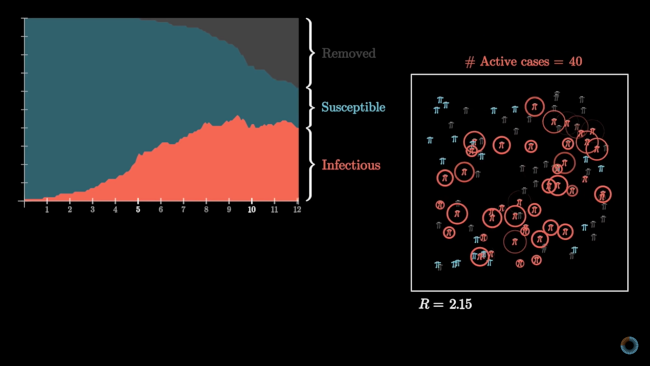
\includegraphics[width=.5\textwidth]{figures/3b1b_covid_agent.png}
        \end{figure}
    \end{itemize}
    \vfill
\end{frame}

\begin{frame}{Examples}
    \vfill
    \begin{itemize}
    \pause
        \item Network based simulations. (covasim)
        \vspace*{.75cm}
                \begin{figure}[H]
                    \centering
                    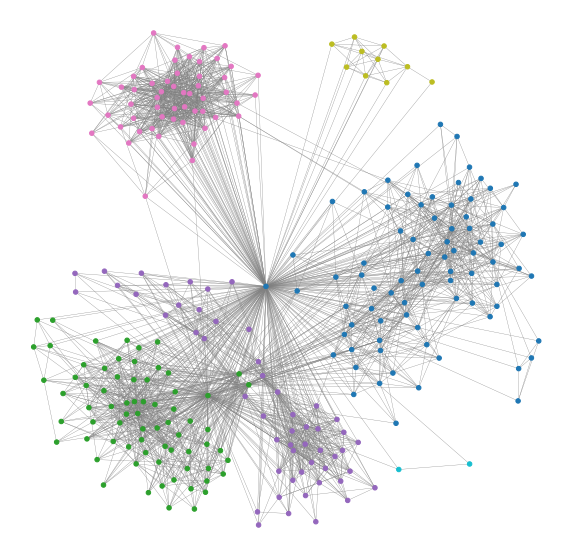
\includegraphics[width=.4\textwidth]{figures/network_diagram.png}
                \end{figure}
            \end{itemize}
            \vfill
\end{frame}

\begin{frame}{Benefits}
    \vfill
    \textbf{\underline{Benefits of agent models:}}
    \begin{itemize}
        \pause
        \item Heterogeneous social structure.
        \pause
        \item Stochastic.
        \pause
        \item (Typically) less ad-hoc parameter tuning.
    \end{itemize}
    \vfill
\end{frame}

\begin{frame}{Drawbacks}
    \vfill
    \textbf{\underline{Drawbacks of agent models:}}
    \begin{itemize}
        \pause
        \item Complicated to design.
        \pause
        \item Slow to run.
        \pause
        \item Stochastic nature requires ensembles to generate statistics.
    \end{itemize}
    \vfill
\end{frame}

\subsection{Compartmental modeling}

\begin{frame}{Compartmental (ODE) based simulations}
    \vfill
    \begin{itemize}
    \pause
        \item Consider an entire homogeneous population.
        \pause
        \item Ignore individualistic behavior for coarse-grained homogeneity.
        \pause
        \item Assume efficient and homogeneous mixing.
    \end{itemize}
    \vfill
\end{frame}

\begin{frame}{Example}
    \vfill
    \begin{itemize}
    \pause
        \item SIR Model (Kermack and McKendrick, 1927)
        \vspace*{1cm}
        \begin{figure}[H]
            \centering
            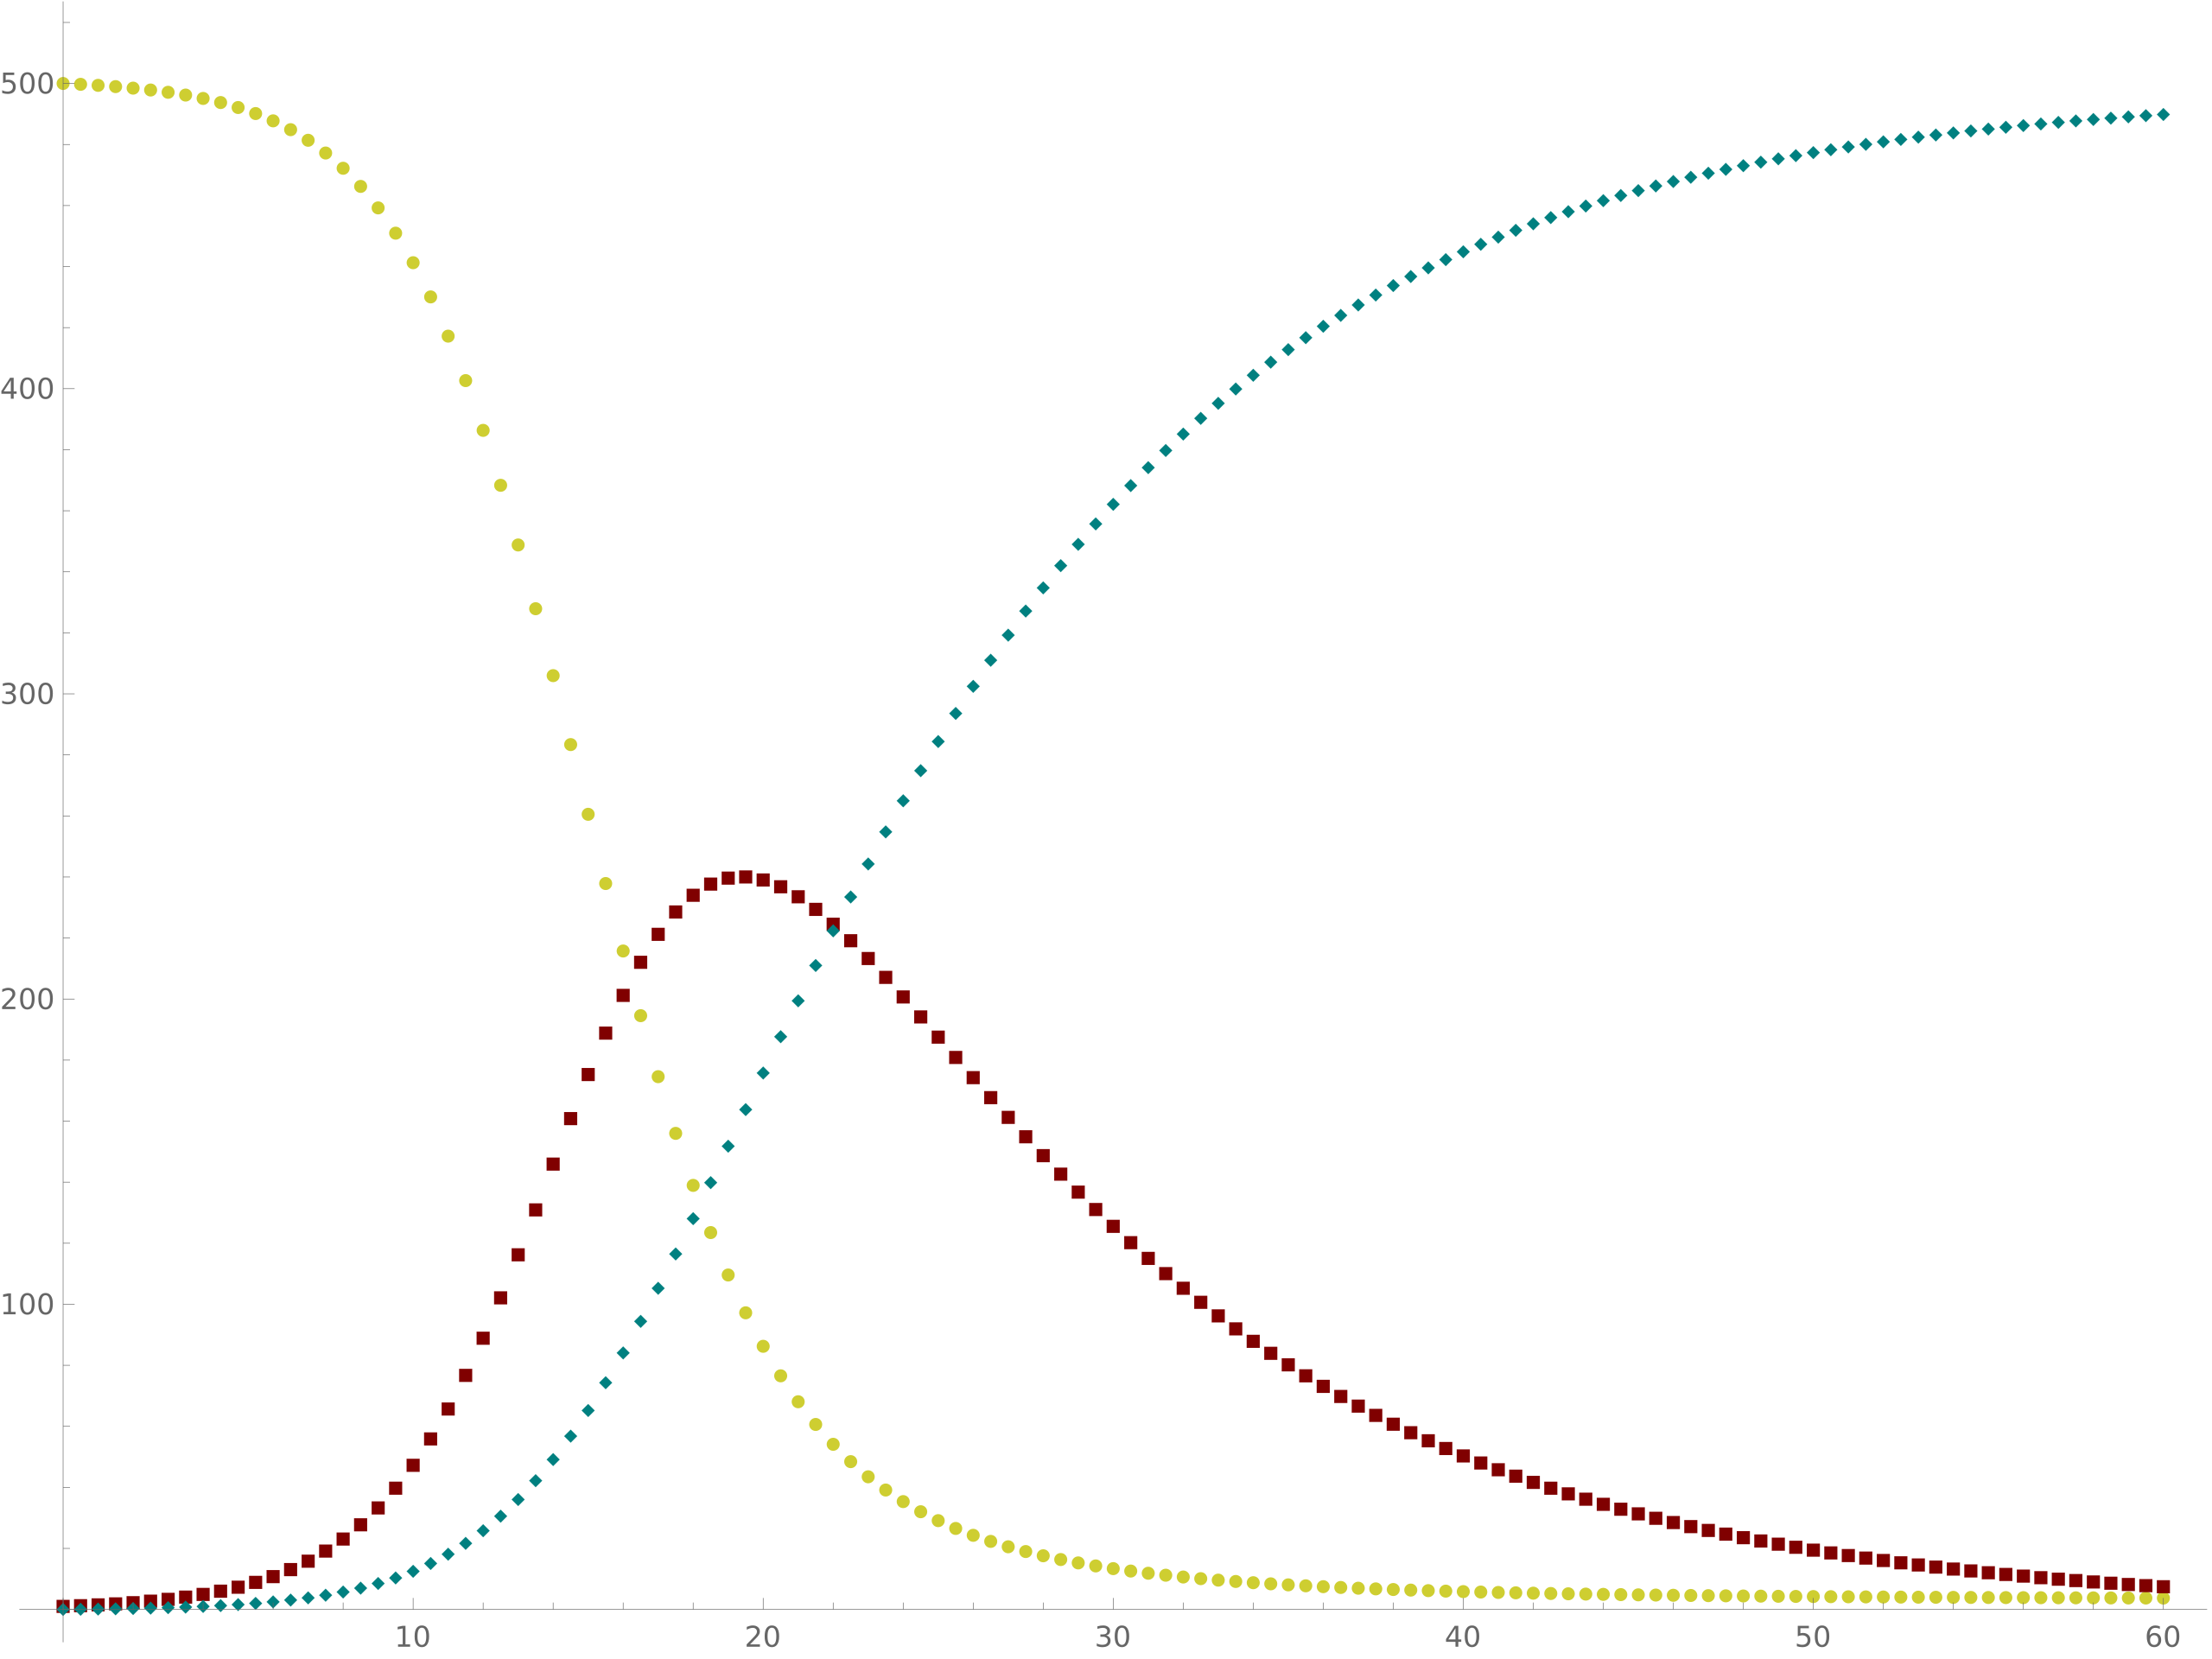
\includegraphics[width=.5\textwidth]{figures/sir_curves.png}
        \end{figure}
    \end{itemize}
    \vfill
\end{frame}

\begin{frame}{SIR equations}
    \vfill
    \pause
    We can write \emph{any} ODE as a first order update of a state $\vecx$ by
    \[
    \xdot = \vecf(t,\vecx).
    \]
    \pause
    The SIR equations then read
    \[
    \begin{pmatrix} \dot{S} \\ \dot{I} \\ \dot{R} \end{pmatrix} = \begin{pmatrix} -\beta C \frac{I}{N} \\ +\beta C \frac{I}{N} - \gamma I \\ + \gamma I \end{pmatrix}, 
    \]
    where $S$, $I$, and $R$ denotes the \boldgreen{susceptible}, \boldgreen{infected}, and \boldgreen{removed} populations respectively. Note, $N=S+I+R$ is the total (conserved) population size.
    \vfill
\end{frame}

\begin{frame}{Relation to chemistry}
\vfill
    The equation
    \[
    \dot{S} = -\beta C \frac{I}{N},
    \]
    can be thought of as a first order chemical reaction
    \[
    S + I \to ...
    \]
    \pause
    \begin{itemize}  
        \item $C$ describes how many contacts with other molecules per unit time species $S$ experiences.
        \pause
        \item $\frac{I}{N}$ is the proportion of these molecules of the proper type.
        \pause
        \item $\beta$ is the likelihood of reaction.
    \end{itemize}
\vfill    
\end{frame}

\begin{frame}{Understanding SIR parameters}
    \vfill
    \pause
    The parameters $\beta$, $C$, and $\gamma$ can be thought of as:
    \begin{itemize}
    \pause
        \item $\beta \in [0,1]$ is likelihood of transmission.
        \pause
        \item $C \in [0,\infty)$ is the contact rate.
        \pause
        \item $\gamma \in [0,\infty)$ is the recovery + death rate.
    \end{itemize}
    \vfill
\end{frame}

\begin{frame}{Benefits}
    \vfill
    \textbf{\underline{Benefits of compartmental models:}}
    \begin{itemize}
        \pause
        \item Easy to build and analyze.
        \pause
        \item Quick to compute.
        \pause
        \item Captures large scale behavior.
    \end{itemize}
    \vfill
\end{frame}

\begin{frame}{Drawbacks}
    \vfill
    \textbf{\underline{Drawbacks of compartmental models:}}
    \begin{itemize}
        \pause
        \item Homogeneous.
        \pause
        \item Deterministic.
        \pause
        \item Ad-hoc parameter changes.
    \end{itemize}
    \vfill
\end{frame}

\subsection{Multiscale modeling}

\begin{frame}{Multiscale modeling}
    \vfill
    \begin{itemize}
    \pause
        \item Interesting dynamics for a single system can take place on various spatio-temporal scales.
        \pause
        \item Small scale interactions drive large scale phenomenon.
        \pause
        \item Couple together small and large scale models to study complicated systems.
        \pause
        \item E.g., quantum mechanics $\to$ molecular dynamics $\to$ kinetic theory $\to$ statistical mechanics $\to$ thermodynamics.
    \end{itemize}
    \vfill
\end{frame}

\begin{frame}{Idea}
    \vfill
    \pause
    Can we couple an agent based model alongside a compartmental model to remove the drawbacks and gain benefits?
    \vfill
\end{frame}

\section{Multiscale COVID-19 modeling}

\subsection{Compartmental model}

\begin{frame}{Hierarchical compartmental model}
\vfill
\pause
Assume the following:
    \begin{itemize}
    \pause
        \item Two coupled SIR systems $S_1$, $I_1$, $R_1$, and $S_2$, $I_2$, and $R_2$.
        \pause
        \item System 1 refers to the university students and System 2 all other citizens in the city that aren't university members.
        \pause
    \end{itemize}
        \begin{figure}[H]
            \centering
            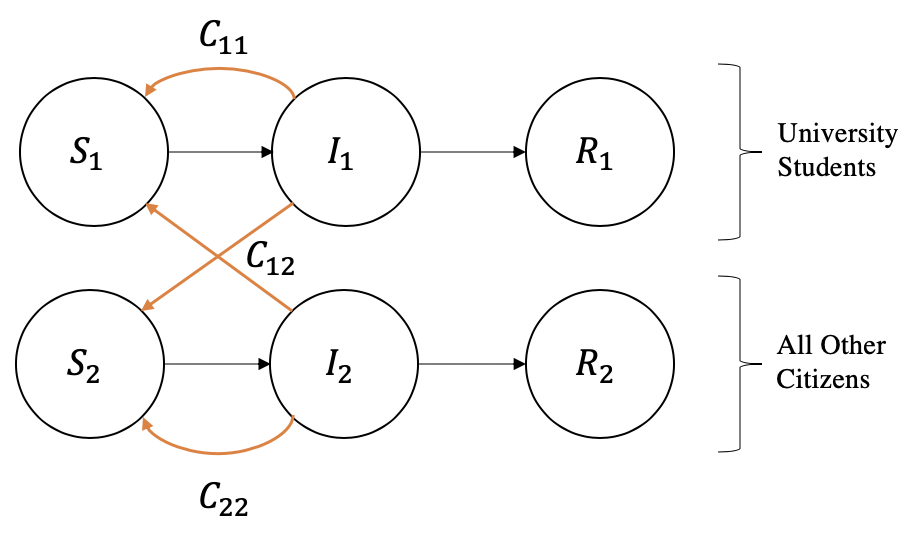
\includegraphics[width=.6\textwidth]{figures/compartmental_sir.png}
        \end{figure}
        \vfill
\end{frame}

\begin{frame}{Hierarchical compartmental model}
\vfill
\pause
    In general, for $n$ systems, we have the equations
    \[
    \begin{pmatrix} \dot{S}_i \\ \dot{I}_i \\ \dot{R}_i \end{pmatrix} = \begin{pmatrix} -\beta S_i \sum_j C_{ij} \frac{I_j}{N_j} \\ +\beta  S_i \sum_j C_{ij} \frac{I_j}{N_j} - \gamma I_j \\ + \gamma I_j \end{pmatrix}.
    \]
    \pause
    In this case, the contact rate $C$ becomes the \boldgreen{contact matrix} $C_{ij}$ that describes the contact rate between the systems $i$ and $j$. Note $C_{ij}$ is symmetric.
    \vfill
\end{frame}

\begin{frame}{Aggregating systems}
    \vfill
    \begin{itemize}
    \pause
    \item Many systems may comprise a larger system (e.g., System 1 + System 2 from before comprise the entire city).
    \pause
    \item This decomposition allows us to aggregate larger system dynamics by summing over relevant systems.
    \end{itemize}
    \vfill
\end{frame}

\begin{frame}{Adding complexity}
\vfill
SIR is lacking.  We prefer the SEQIRD compartmental model governed by
\begin{columns}
\begin{column}{0.5\textwidth}
\[
\begin{pmatrix} \dot{S}_i \\ \dot{E}_i \\ \dot{Q}_i \\ \dot{I}_i \\ \dot{R}_i \\ \dot{D}_i \end{pmatrix} = \begin{pmatrix} -\beta S_i \sum_j C_{ij} \frac{I_j}{N_j} \\ \beta S_i \sum_j C_{ij} \frac{I_j}{N_j} - (\gamma_I - \gamma_Q)E_i \\ \gamma_I E_i - (\lambda + \kappa)I_i \\ \gamma_Q E_i - (\lambda + \kappa) Q_i \\ \lambda(I_i + Q_i) \\ \kappa (I_i + Q_i) \end{pmatrix}
\]
\end{column}
\begin{column}{0.5\textwidth}
    \begin{itemize}
        \item $S \equiv $ susceptible.
        \item $E \equiv $ exposed.
        \item $Q \equiv $ quarantined.
        \item $I \equiv $ infected.
        \item $R \equiv $ recovered.
        \item $D \equiv $ dead.
    \end{itemize}
\end{column}
\end{columns}
\vfill
\end{frame}

\begin{frame}{Adding complexity}
\vfill
SIR is lacking.  We prefer the SEQIRD compartmental model governed by
\begin{columns}
\begin{column}{0.5\textwidth}
\[
\begin{pmatrix} \dot{S}_i \\ \dot{E}_i \\ \dot{Q}_i \\ \dot{I}_i \\ \dot{R}_i \\ \dot{D}_i \end{pmatrix} = \begin{pmatrix} -\beta S_i \sum_j C_{ij} \frac{I_j}{N_j} \\ \beta S_i \sum_j C_{ij} \frac{I_j}{N_j} - (\gamma_I - \gamma_Q)E_i \\ \gamma_I E_i - (\lambda + \kappa)I_i \\ \gamma_Q E_i - (\lambda + \kappa) Q_i \\ \lambda(I_i + Q_i) \\ \kappa (I_i + Q_i) \end{pmatrix}
\]
\end{column}
\begin{column}{0.5\textwidth}
    \begin{itemize}
        \item $\beta = 0.3 \equiv $ transmission rate.
        \item $C \equiv $ contact matrix.
        \item $\gamma = 0.07 \equiv $ latent time to infection.
        \item $\lambda = 0.1 \equiv $ recovery rate.
        \item $\kappa = 0.002 \equiv $ death rate.
        \item $q_{\textrm{percent}} \equiv $ percentage quarantining.
        \item $\gamma_Q = q_{\textrm{percent}} \gamma$.
        \item $\gamma_I = (1-q_{\textrm{percent}}) \gamma$.
    \end{itemize}
\end{column}
\end{columns}
\vfill
\end{frame}

\begin{frame}{Determining parameters}
    \vfill
    \pause
        \begin{figure}[H]
            \centering
            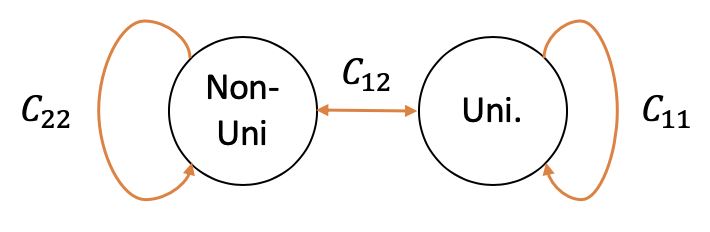
\includegraphics[width=.5\textwidth]{figures/contact_diagram.png}
        \end{figure}
    \begin{itemize}
\item    All parameters but $C$ were determined via measurements in other sources.
\pause
\item We determine the values for $C$ via data assimilation and a agent based model.
\pause
\item \boldgreen{This is where the model becomes multiscale.}
    \end{itemize}
\end{frame}

\begin{frame}{Assimilating data}
    \vfill
    \pause
    Using measured data from Fort Collins and Larimer County, we estimated a value for $C$ assuming $\beta=1$.
    \begin{figure}[H]
    \centering
    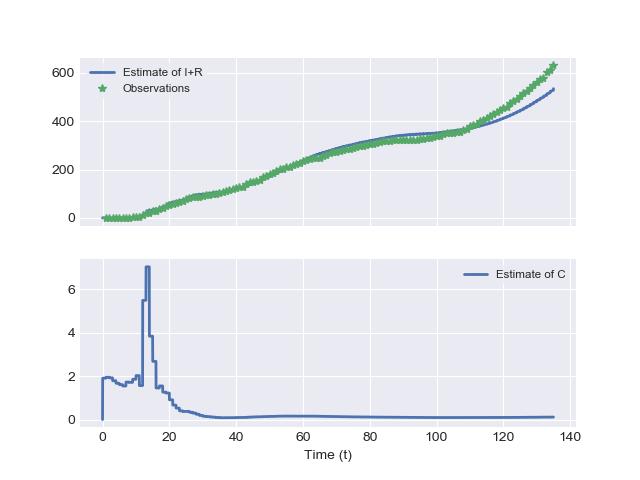
\includegraphics[width=.6\textwidth]{figures/data_assimilation.png}
    \end{figure}
    \pause
    We're working on improving this estimate with newer data with more adequate assimilation techniques (optimal proposal particle filtering as opposed to ensemble Kalman filtering).
    \vfill
\end{frame}

\subsection{Agent model}

\begin{frame}{Counting contacts}
    \vfill
    \pause
    \begin{columns}
    \begin{column}{.5\textwidth}
    \textbf{\underline{Idea:}} Agent based simulator tracks (various types of) contact between students each day.\\
    \vspace*{1cm}
    \textbf{\underline{Adjustable parameters:}}
    \begin{itemize}
        \item Student body size.
        \item Number of class periods.
        \item Class sizes.
        \item Students per major.
        \item Schedule staggering.
    \end{itemize}
    \end{column}
    \begin{column}{.5\textwidth}
        \begin{figure}[H]
            \centering
            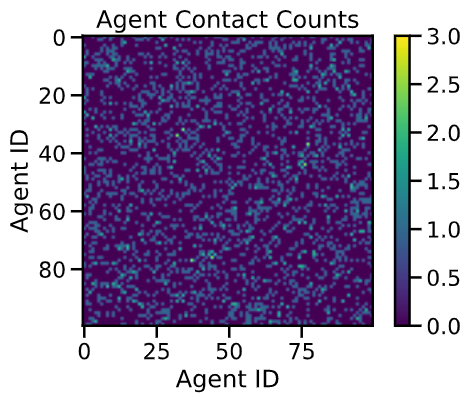
\includegraphics[width=\textwidth]{figures/contact_matrix.png}
        \end{figure}
    \end{column}
    \end{columns}
    \vfill
\end{frame}


\begin{frame}{Contacts and school population}
    \vfill
    \begin{columns}
    \begin{column}{.4\textwidth}
        \begin{itemize}

            \item Students are randomly assigned courses of a certain size.

            \item We count the number of unique contacts a student makes vs. class size for a three class period day.

            \item The growth is sublinear, but as the population increases we approach linear behavior.

            \item This is due to diminishing chances of having repeat students in other randomly drawn classes.
        \end{itemize}
    \end{column}
    \begin{column}{.6\textwidth}
        \begin{figure}[H]
            \centering
            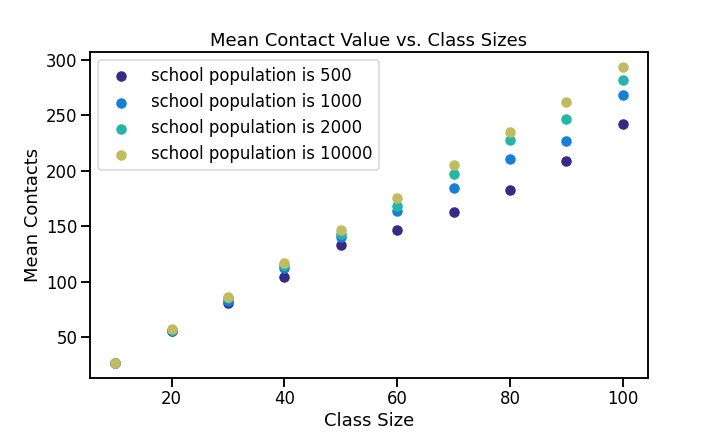
\includegraphics[width=\textwidth]{figures/contacts_vs_population.png}
        \end{figure}
    \end{column}
    \end{columns}
    \vfill
\end{frame}

\begin{frame}{Contacts and major grouping}
    \vfill
    \begin{columns}
    \begin{column}{.3\textwidth}
        \begin{itemize}
            \item To add realism or intervention, we can group students within majors.
            \item This leads to a decrease in new contacts and sublinear growth due to the effective population size decreasing to the size of the majors (500).
        \end{itemize}
    \end{column}
    \begin{column}{.7\textwidth}
        \begin{figure}[H]
            \centering
            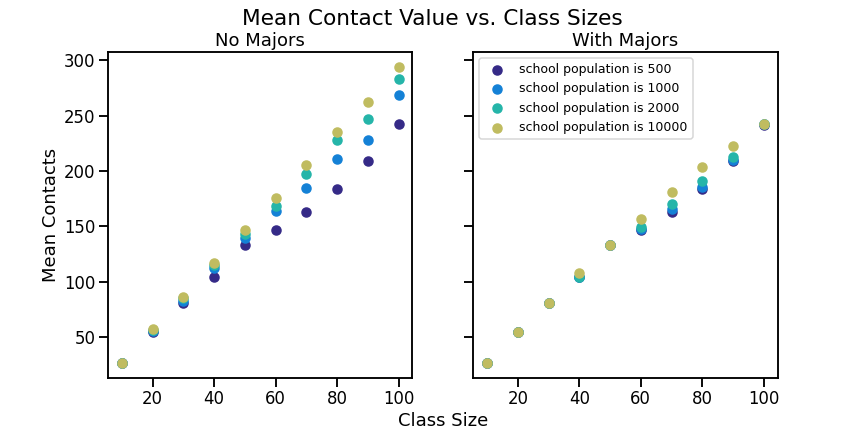
\includegraphics[width=\textwidth]{figures/contacts_vs_population_majors.png}
        \end{figure}
    \end{column}
    \end{columns}
    \vfill
\end{frame}

\begin{frame}{Contacts and class periods}
    \vfill
    \begin{columns}
    \begin{column}{.3\textwidth}
        \begin{itemize}
            \item Increasing the number of in-person class periods increases contact rate almost linearly when class sizes are small (30).
        \end{itemize}
    \end{column}
    \begin{column}{.7\textwidth}
        \begin{figure}[H]
            \centering
            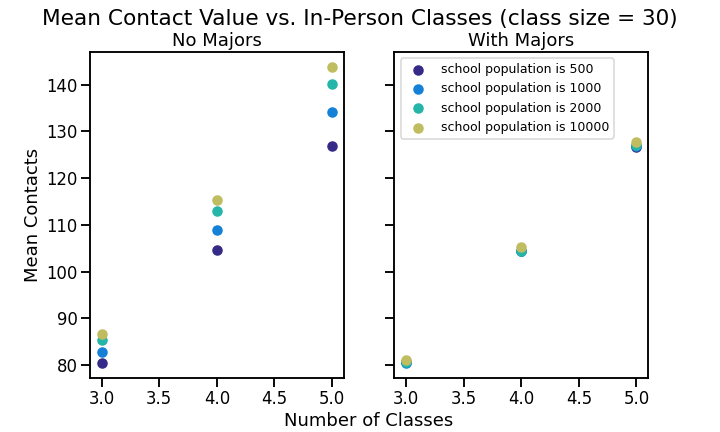
\includegraphics[width=\textwidth]{figures/contacts_vs_periods.png}
        \end{figure}
    \end{column}
    \end{columns}
    \vfill
\end{frame}

\begin{frame}{Integrating the agent model}
    \vfill
    \begin{itemize}
    \pause
    \item At the beginning of each day, the agent model is ran to compute a contact rate within the university.
    \pause
    \item This contact rate is used in the compartmental model and we integrate this ODE for a day.
    \pause 
    \item University members in the Q and D department are removed and the contact rate is recomputed
    \end{itemize}
    \vfill
\end{frame}

\begin{frame}{City-university coupling}
    \vfill
    \begin{columns}
    \begin{column}{.3\textwidth}
        \begin{itemize}
            \item City-university coupling changes the strength of the off diagonal $C_{21}$ element.
            \item With high coupling, $C_{21}=C_{22}$ and students mix just like typical city members.
            \item Coupling minimally affects the university, but greatly affects the city.
        \end{itemize}
    \end{column}
    \begin{column}{.7\textwidth}
        \begin{figure}[H]
            \centering
            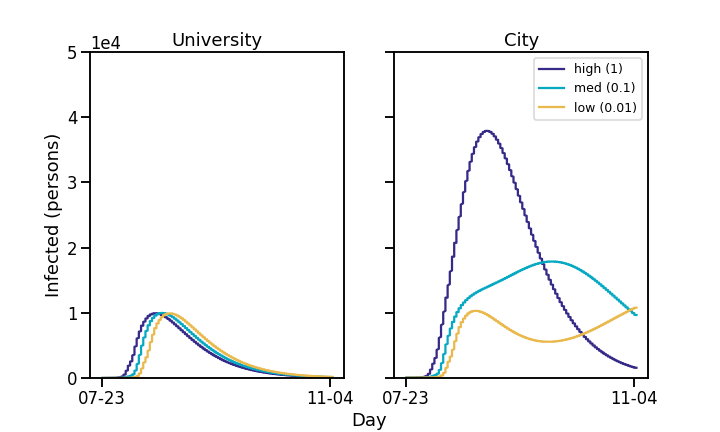
\includegraphics[width=\textwidth]{figures/city_university_coupling.png}
            \caption{$I(t)$ for class size = 15, major size = 500, and no quarantining.}
        \end{figure}
    \end{column}
    \end{columns}
    \vfill
\end{frame}

\begin{frame}{University quarantining}
    \begin{columns}
    \begin{column}{.3\textwidth}
    \vfill
        \begin{itemize}
            \item Quarantining only delays infection within the university.
            \item Significantly alters aggregated city dynamics and prevents second wave.
        \end{itemize}
        \vfill
    \end{column}
    \begin{column}{.7\textwidth}
    \vfill
        \begin{figure}[H]
            \centering
            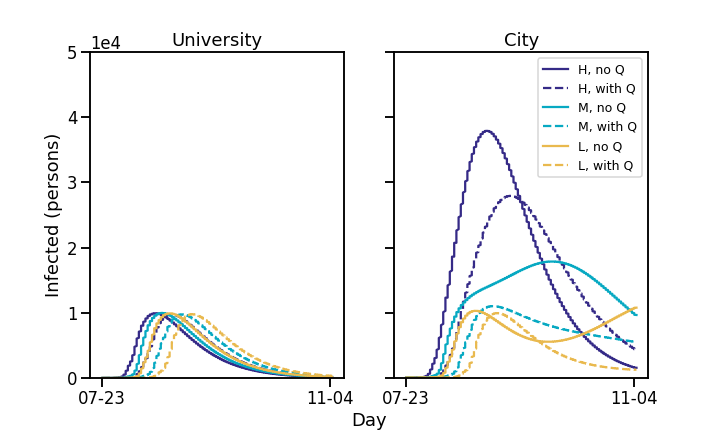
\includegraphics[width=\textwidth]{figures/university_quarantining.png}
            \caption{$I(t)$ with 50\% quarantine rate, class size of 15, and major size = 500.}
        \end{figure}
        \vfill
    \end{column}
    \end{columns}
\end{frame}

\begin{frame}{Staggering schedules}
    \vfill
    \begin{columns}
    \begin{column}{.3\textwidth}
        \begin{itemize}
            \item Day and week staggering flatten the curve and reduce total infected.
            \item Week staggering performs slightly better due to latent time for infection.
        \end{itemize}
    \end{column}
    \begin{column}{.7\textwidth}
        \begin{figure}[H]
            \centering
            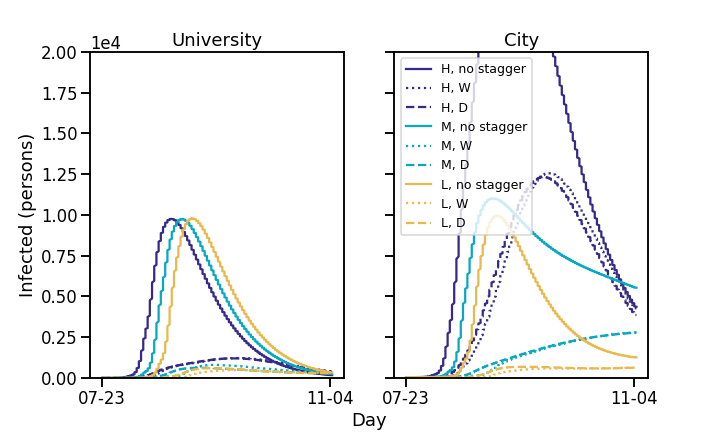
\includegraphics[width=\textwidth]{figures/staggering_schedules.png}
            \caption{$I(t)$ with staggering, 50\% of infected population quarantining, class size = 15, major size = 500.}
        \end{figure}
    \end{column}
    \end{columns}
    \vfill
\end{frame}

\begin{frame}{Future directions}
    \vfill
    \begin{itemize}
        \item Improve and extend the data assimilation for the compartmental model.
        \item Incorporate different types of contacts.
        \item Masks, hygiene, and other measures of contact severity.
        \item Quantify the stochasticity of the agent model.
        \item More heterogeneity from the agent model (scheduling, transportation, etc.).
    \end{itemize}
    \vfill
\end{frame}



%%%%%%%%%%%%%%%%%%%%%%%%%%%%%%%%%%%%%%%%%%%%%%%%%%%%%%%%%%%%%%%%%%%%%%%%%%%%%%%%%%%%%%%%%%%%%%%

\begin{frame}{Acknowledgements}
\vfill
\begin{figure}
     \centering
     \begin{subfigure}[b]{0.35\textwidth}
         \centering
         
\includegraphics[width=\textwidth]{figures/mcrn_logo.png}
     \end{subfigure}
     \hspace*{2cm}
     \begin{subfigure}[b]{0.23\textwidth}
         \centering
         
\includegraphics[width=\textwidth]{figures/nsf_logo.png}
     \end{subfigure}
     \\
     \vspace*{1cm}
     \begin{subfigure}[b]{0.7\textwidth}
         \centering
         
\includegraphics[width=\textwidth]{figures/aim_logo.jpg}
     \end{subfigure}
\end{figure}
\vfill
\end{frame}




\end{document}